% ***************************************************************************************************
%
%	Praca inżynierska:
%	Autor:	Tomasz Kulik
%
% ***************************************************************************************************

% Styl dwustronny z domyślną wielkością czcionki 10pt oraz oddzieloną stroną tytułową (titlepage).
% Domyślnie rodziały rozpoczynają się na stronie prawej (openright).
\documentclass{book}

% ***************************************************************************************************
% Ustawienia języka
% ***************************************************************************************************

\usepackage[polish]{babel}

% Pakiet babel dla polskiego języka powoduje konflikt z pakietem amssymb.
% Polecenie '\lll' definiują oba pakiety - porządana jest druga definicja.
\let\lll\undefined

\selectlanguage{polish}
\usepackage[utf8]{inputenc}
\usepackage{lmodern}

\usepackage{indentfirst}
\usepackage[plmath]{polski}
\usepackage{icomma}
\frenchspacing
\usepackage{amsmath}
\usepackage{amssymb}
\usepackage{mathrsfs}

% Dodatkowe wsparcie dla środowiska mathbb, które nie wspiera domyślnie cyfr (\mathbb{})
\usepackage{bbold}
\usepackage{mathtools}


% ***************************************************************************************************
% Kolory
% ***************************************************************************************************

% Umożliwia kolorowanie poszczególnych komórek tabeli
\usepackage[table]{xcolor}% http://ctan.org/pkg/

% Umożliwia łatwą zmianę koloru linii w tabeli
\usepackage{tabu}

% Umożliwia rozszerzoną kontrolę nad kolorami.
\usepackage{xcolor}

% Definicje kolorów
\definecolor{lgray}{HTML}{9F9F9F}
\definecolor{dgray}{HTML}{5F5F5F}
% lgray				-	nazwa nowo zdefiniowanego koloru
% HTML				-	model kolorów
% CCCCCC			-	wartość koloru zgodna z modelem

% ***************************************************************************************************
% Algorytmy
% ***************************************************************************************************

% Udostępnia środowisko do konstruowania pseudokodów
\usepackage[ruled,vlined,linesnumbered,longend,algochapter]{algorithm2e}
% ruled	- poziome kreski na początku i końcu algorytmu, podpis na górze oddzielony również kreską poziomą
% vlined - pionowe kreski łączące początek polecenia z jego końcem
% linesnumbered	- numerowanie kolejnych wierszy algorytmu
% longend - długie końcówki np. ifend, forend itd.
% algochapter - numeracja z rozdziałami

% Zamiana nazwy środowiska z domyślnej "Algorithm X" na "Pseudokod X"
\newenvironment{pseudokod}[1][htb]{
        \renewcommand{\algorithmcfname}{Pseudokod}
        \begin{algorithm}[#1]%
        }{
\end{algorithm}
}

% Zmiana rozmiaru komentarzy
\newcommand\algcomment[1]{
        \footnotesize{#1}
}

% Ustawienie zadanego stylu dla komentarzy
\SetCommentSty{algcomment}

\usepackage{textcomp}%
\newcommand{\textapprox}{\raisebox{0.5ex}{\texttildelow}}

\usepackage{listings}
\renewcommand{\lstlistingname}{Kod źródłowy}

% Definicje pecjalnych znaków, które nie są obsługiwane w środowisku listing
\lstset{literate=
        {ż}{{\.{z}}}1	{ź}{{\'{z}}}1
        {ć}{{\'{c}}}1	{ń}{{\'{n}}}1
        {ą}{{\c a}}1	{ś}{{\'{s}}}1
        {ł}{{\l}}1		{ę}{{\c{e}}}1
        {ó}{{\'{o}}}1	{á}{{\'a}}1
        {é}{{\'e}}1		{í}{{\'i}}1
        {ó}{{\'o}}1		{ú}{{\'u}}1
        {ù}{{\`u}}1		{Á}{{\'A}}1
        {É}{{\'E}}1		{Í}{{\'I}}1
        {Ó}{{\'O}}1		{Ú}{{\'U}}1
        {à}{{\`a}}1		{è}{{\'e}}1
        {ì}{{\`i}}1		{ò}{{\`o}}1
        {ò}{{\`o}}1		{À}{{\`A}}1
        {È}{{\'E}}1		{Ì}{{\`I}}1
        {Ò}{{\`O}}1		{Ò}{{\`O}}1
        {ä}{{\"a}}1		{ë}{{\"e}}1
        {ï}{{\"i}}1		{ö}{{\"o}}1
        {ü}{{\"u}}1		{Ä}{{\"A}}1
        {Ë}{{\"E}}1		{Ï}{{\"I}}1
        {Ö}{{\"O}}1		{Ü}{{\"U}}1
        {â}{{\^a}}1		{ê}{{\^e}}1
        {î}{{\^i}}1		{ô}{{\^o}}1
        {û}{{\^u}}1		{Â}{{\^A}}1
        {Ê}{{\^E}}1		{Î}{{\^I}}1
        {Ô}{{\^O}}1		{Û}{{\^U}}1
        {œ}{{\oe}}1		{Œ}{{\OE}}1
        {æ}{{\ae}}1		{Æ}{{\AE}}1
        {ß}{{\ss}}1		{ç}{{\c c}}1
        {Ç}{{\c C}}1	{ø}{{\o}}1
        {å}{{\r a}}1	{Å}{{\r A}}1
        {€}{{\EUR}}1	{£}{{\pounds}}1
}

% ***************************************************************************************************
% Marginesy
% ***************************************************************************************************

% Ustawienia rozmiarów stron i ich marginesów
\usepackage[headheight=18pt, top=25mm, bottom=25mm, left=25mm, right=25mm]{geometry}
% headheight		-	wysokość tytułów
% top				-	margines górny
% bottom			-	margines dolny
% left				-	margines lewy
% right				-	margines prawy

% Usunięcie górnego marginesu dla środowisk
\makeatletter
\setlength\@fptop{0\p@}
\makeatother

% ***************************************************************************************************
% Styl
% ***************************************************************************************************

% Definiuje środowisko 'titlingpage', które zapewnia pełną kontrolę nad układem strony tytułowej.
\usepackage{titling}


% Umożliwia modyfikowanie stylu spisu treści
\usepackage{tocloft}

\tocloftpagestyle{tableOfContentStyle}

% Definiowanie własnych stylów nagłówków i/lub stopek
\usepackage{fancyhdr}

% Domyślny styl dla pracy
\fancypagestyle{custom}{
        \fancyhf{}									% wyczyść stopki i nagłówki
        \fancyhead[RO]{								% Prawy, nieparzysty nagłówek
                \hrulefill \hspace{16pt} \large Rozdział \thechapter
                \put(-472.1, 12.1){%
                        \makebox(0,0)[l]{%
                                
\includegraphics[width=0.05\textwidth]{pwr-logo}
                        }
                }
                \put(-443,5.5){%
                        \makebox(0,0)[l]{%
                                \small Politechnika Wrocławska
                        }
                }
        }
        \fancyhead[LE]{								% Lewy, parzysty nagłówek
                \large Rozdział \thechapter \hspace{16pt} \hrulefill
                \put(-22, 12.1){%
                        \makebox(0,0)[l]{%
                                
\includegraphics[width=0.05\textwidth]{wppt-logo}
                        }
                }
                \put(-210,5.5){%
                        \makebox(0,0)[l]{%
                                \small Wydział Podstawowych Problemów Techniki
                        }
                }
        }
        \fancyfoot[LE,RO]{							% Stopki
                \thepage
        }
        \renewcommand{\headrulewidth}{0pt}			% Grubość linii w nagłówku
        \renewcommand{\footrulewidth}{0.2pt}		% Grubość linii w stopce
}


% Domyślny styl dla bibliografii
\fancypagestyle{bibliographyStyle}{
        \fancyhf{}									% wyczyść stopki i nagłówki
        \fancyhead[RO]{								% Prawy, nieparzysty nagłówek
                \hrulefill \hspace{16pt} \large Dodatek \thechapter
                \put(-472.1, 12.1){%
                        \makebox(0,0)[l]{%
                                
\includegraphics[width=0.05\textwidth]{pwr-logo}
                        }
                }
                \put(-443,5.5){%
                        \makebox(0,0)[l]{%
                                \small Politechnika Wrocławska
                        }
                }
        }
        \fancyhead[LE]{								% Lewy, parzysty nagłówek
                \large Bibliografia \hspace{16pt} \hrulefill
                \put(-22, 12.1){%
                        \makebox(0,0)[l]{%
                                
\includegraphics[width=0.05\textwidth]{wppt-logo}
                        }
                }
                \put(-210,5.5){%
                        \makebox(0,0)[l]{%
                                \small Wydział Podstawowych Problemów Techniki
                        }
                }
        }
        \fancyfoot[LE,RO]{							% Stopki
                \thepage
        }
        \renewcommand{\headrulewidth}{0pt}			% Grubość linii w nagłówku
        \renewcommand{\footrulewidth}{0.2pt}		% Grubość linii w stopce
}

% Domyślny styl dla dodatków
\fancypagestyle{appendixStyle}{
        \fancyhf{}									% wyczyść stopki i nagłówki
        \fancyhead[RO]{								% Prawy, nieparzysty nagłówek
                \hrulefill \hspace{16pt} \large Dodatek \thechapter
                \put(-472.1, 12.1){%
                        \makebox(0,0)[l]{%
                                
\includegraphics[width=0.05\textwidth]{pwr-logo}
                        }
                }
                \put(-443,5.5){%
                        \makebox(0,0)[l]{%
                                \small Politechnika Wrocławska
                        }
                }
        }
        \fancyhead[LE]{								% Lewy, parzysty nagłówek
                \large Dodatek \thechapter \hspace{16pt} \hrulefill
                \put(-22, 12.1){%
                        \makebox(0,0)[l]{%
                                
\includegraphics[width=0.05\textwidth]{wppt-logo}
                        }
                }
                \put(-210,5.5){%
                        \makebox(0,0)[l]{%
                                \small Wydział Podstawowych Problemów Techniki
                        }
                }
        }
        \fancyfoot[LE,RO]{							% Stopki
                \thepage
        }
        \renewcommand{\headrulewidth}{0pt}			% Grubość linii w nagłówku
        \renewcommand{\footrulewidth}{0.2pt}		% Grubość linii w stopce
}

% Osobny styl dla stron zaczynających rozdział/spis treści itd. (domyślnie formatowane jako "plain")
\fancypagestyle{chapterBeginStyle}{
        \fancyhf{}%
        \fancyfoot[LE,RO]{
                \thepage
        }
        \renewcommand{\headrulewidth}{0pt}
        \renewcommand{\footrulewidth}{0.2pt}
}

% Styl dla pozostałych stron spisu treści
\fancypagestyle{tableOfContentStyle}{
        \fancyhf{}%
        \fancyfoot[LE,RO]{
                \thepage
        }
        \renewcommand{\headrulewidth}{0pt}
        \renewcommand{\footrulewidth}{0.2pt}
}

% Formatowanie tytułów rozdziałów i/lub sekcji
\usepackage{titlesec}

% Formatowanie tytułów rozdziałów
\titleformat{\chapter}[hang]					% kształt
{
        \vspace{-10ex}
        \Huge
        \bfseries
}												% formatowanie tekstu modyfikowanego elementu
{}												% etykieta występująca przed tekstem modyfikowanego elementu, niewidoczna w spisie treści
{
        10pt
}												% odstęp formatowanego tytułu od lewego marginesu/etykiety
{
        \Huge
        \bfseries
}												% formatowanie elementów przed modyfikowanym tytułem
[
\vspace{2ex}
%\rule{\textwidth}{0.4pt}
%\vspace{-4ex}
]												% dodatkowe formatowanie stosowane poniżej modyfikowanego tytułu


% Formatowanie tytułów sekcji
\titleformat{\section}[hang]					% kształt
{
        \vspace{2ex}
%	\titlerule\vspace{1ex}
        \Large\bfseries
}												% formatowanie tekstu modyfikowanego elementu
{
        \thesection									% etykieta występująca przed tekstem modyfikowanego elementu, niewidoczna w spisie treści
}
{
        0pt
}												% odstęp formatowanego tytułu od lewego marginesu/etykiety
{
        \Large
        \bfseries
}												% formatowanie elementów przed modyfikowanym tytułem

% ***************************************************************************************************
% Linki
% ***************************************************************************************************

% Umożliwia wstawianie hiperłączy do dokumentu
\usepackage{hyperref}							% Aktywuje linki

\hypersetup{
        colorlinks	=	true,					% Koloruje tekst zamiast tworzyć ramki.
        linkcolor		=	blue,					% Kolory: referencji,
        citecolor		=	blue,					% cytowań,
        urlcolor		=	blue					% hiperlinków.
}

% Do stworzenia hiperłączy zostanie użyta ta sama (same) czcionka co dla reszty dokumentu
\urlstyle{same}




% ***************************************************************************************************
% Linki
% ***************************************************************************************************

% Umożliwia zdefiniowanie własnego stylu wyliczeniowego
\usepackage{enumitem}

% Nowa lista numerowana z trzema poziomami
\newlist{myitemize}{itemize}{3}

% Definicja wyglądu znacznika pierwszego poziomu
\setlist[myitemize,1]{
        label		=	\textbullet,
        leftmargin	=	4mm}

% Definicja wyglądu znacznika drugiego poziomu
\setlist[myitemize,2]{
        label		=	$\diamond$,
        leftmargin	=	8mm}

% Definicja wyglądu znacznika trzeciego poziomu
\setlist[myitemize,3]{
        label		=	$\diamond$,
        leftmargin	=	12mm
}

% ***************************************************************************************************
% Inne pakiety
% ***************************************************************************************************

% Dołączanie rysunków
\usepackage{graphicx}

% Figury i przypisy
\usepackage{caption}
\usepackage{subcaption}

% Umożliwia tworzenie przypisów wewnątrz środowisk
\usepackage{footnote}

% Umożliwia tworzenie struktur katalogów
\usepackage{dirtree}

% Rozciąganie komórek tabeli na wiele wierszy
\usepackage{multirow}

% Precyzyjne obliczenia szerokości/wysokości dowolnego fragmentu wygenerowanego przez LaTeX
\usepackage{calc}

% ***************************************************************************************************
% Matematyczne skróty
% ***************************************************************************************************

% Skrócony symbol liczb rzeczywistych
\newcommand{\RR}{\mathbb{R}}

% Skrócony symbol liczb naturalnych
\newcommand{\NN}{\mathbb{N}}

% Skrócony symbol liczb wymiernych
\newcommand{\QQ}{\mathbb{Q}}

% Skrócony symbol liczb całkowitych
\newcommand{\ZZ}{\mathbb{Z}}

% Skrócony symbol logicznej implikacji
\newcommand{\IMP}{\rightarrow}

% Skrócony symbol  logicznej równoważności
\newcommand{\IFF}{\leftrightarrow}

% ***************************************************************************************************
% Środowiska
% ***************************************************************************************************

% Środowisko do twierdzeń
\newtheorem{theorem}{Twierdzenie}[chapter]

% Środowisko do lematów
\newtheorem{lemma}{Lemat}[chapter]

% Środowisko do przykładów
\newtheorem{example}{Przykład}[chapter]

% Środowisko do wniosków
\newtheorem{corollary}{Wniosek}[chapter]

% Środowisko do definicji
\newtheorem{definition}{Definicja}[chapter]

% Środowisko do dowodów
\newenvironment{proof}{
        \par\noindent \textbf{Dowód.}
}{
\begin{flushright}
        \vspace*{-6mm}\mbox{$\blacklozenge$}
\end{flushright}
}

% Środowisko do uwag
\newenvironment{remark}{
        \bigskip \par\noindent \small \textbf{Uwaga.}
}{
\begin{small}
        \vspace*{4mm}
\end{small}
}

% ***************************************************************************************************
% Słownik
% ***************************************************************************************************

% Prawidłowe dzielenie wyrazów
\hyphenation{wszy-stkich ko-lu-mnę każ-da od-leg-łość
        dzie-dzi-ny dzie-dzi-na rów-nych rów-ny
        pole-ga zmie-nna pa-ra-met-rów wzo-rem po-cho-dzi
        o-trzy-ma wte-dy wa-run-ko-wych lo-gicz-nie
        skreś-la-na skreś-la-ną cał-ko-wi-tych wzo-rów po-rzą-dek po-rząd-kiem
        przy-kład pod-zbio-rów po-mię-dzy re-pre-zen-to-wa-ne
        rów-no-waż-ne bi-blio-te-kach wy-pro-wa-dza ma-te-ria-łów
        prze-ka-za-nym skoń-czo-nym moż-esz na-tu-ral-na cią-gu tab-li-cy
        prze-ka-za-nej od-po-wied-nio}

% ***************************************************************************************************
% Dokument
% ***************************************************************************************************

\frontmatter

\begin{document}

        \begin{titlingpage}
                \vspace*{\fill}
                \begin{center}
                        \begin{picture}(300,510)
                                \put(11,520){\makebox(0,0)[l]{\large \textsc{Wydział Podstawowych Problemów Techniki}}}
                                \put(11,500){\makebox(0,0)[l]{\large \textsc{Politechnika Wrocławska}}}
% Tytuł pracy
%Komputerowe modelowanie i rozwiązywanie geometrycznych łamigłówek wymagających detekcji kolizji
                                \put(40,320){\LARGE \textsc{Komputerowe modelowanie i rozwiązywanie}}
                                \put(40,290){\LARGE \textsc{geometrycznych łamigłówek wymagających}}
                                \put(40,260){\LARGE \textsc{detekcji kolizji}}
% Autor pracy
                                \put(90,200){\makebox(0,0)[l]{\large \textsc{Tomasz Kulik}}}
                                \put(90,180){\makebox(0,0)[l]{\large \textsc{Nr indeksu: 208869}}}

                                \put(200,100){\makebox(0,0)[l]{\large Praca inżynierska napisana}}
                                \put(200,80){\makebox(0,0)[l]{\large pod kierunkiem}}
% dane promotora
                                \put(200,60){\makebox(0,0)[l]{\large doktora Przemysława Kobylańskiego}}

                                \put(115,-70){
\includegraphics[width=0.15\textwidth]{pwr}}
                                \put(106,-80){\makebox(0,0)[bl]{\large \textsc{Wrocław 2017}}}
                        \end{picture}
                \end{center}
                \vspace*{\fill}
        \end{titlingpage}

        \cleardoublepage

        \pagenumbering{Roman}
        \pagestyle{tableOfContentStyle}
        \tableofcontents
        \cleardoublepage

        % ***************************************************************************************************
        % Wstęp
        % ***************************************************************************************************

        \pagestyle{custom}
        \mainmatter

        % ***************************************************************************************************
        % Rodziały
        % ***************************************************************************************************

        \chapter{Wstęp}
\thispagestyle{chapterBeginStyle}
Zagadki zdają się być dziedziną przeznaczoną głównie dla osób młodych. Wiele z nich pozytywnie wpływa na rozwój człowieka, pobudza jego wyobraźnię oraz uczy logicznego myślenia. Człowiek z natury rozumny jest w stanie wymyślać i rozwiązywać tego typu problemy. Zadanie komplikuje się, jeśli takie zagadki miałaby rozwiązywać maszyna. Bowiem ilość możliwych do sprawdzenia kombinacji często przekracza możliwości współczesnych komputerów. Aby umożliwić w pewnym tylko stopniu rozwiązywanie takich  problemów przez algorytmy komputerowe, należy nałożyć odpowiednie ograniczenia na model, co wiąże się z redukcją liczby kombinacji i możliwością wprowadzenia odpowiednich optymalizacji. Problemów wymagających analizy geometrycznej jest wiele. Szczególnym typem łamigłówek są te złożone z mniejszych elementów, które odpowiednio ułożone tworzą pewne bryły. Ciekawym przykładem jest zagadka polegająca na stworzeniu sześcianu przy pomocy połączonych ze sobą mniejszych klocków. Motywacją do napisania niniejszej pracy było przełamanie kolejnej bariery, dokładna analiza problemu oraz rozwikłanie zagadki, w tym przypadku algorytmicznej.

Celem pracy jest napisanie aplikacji do rozwiązywania łamigłówek geometrycznych złożonych z połączonych ze sobą sześcianów.

W zakres prac wchodzi zaprojektowanie aplikacji niezależnej od platformy, której działanie jest skupione na rozwiązywaniu wspomnianych łamigłówek. Aplikacja ma następujące założenia:
\begin{itemize}
\item generowanie modelu,
\item rozwiązywanie postawionego problemu,
\item prezentacja wyniku.
\end{itemize}

Praca składa się z czterech rozdziałów. W każdym rozdziale znajduje się dokładny opis przedmiotu, którego dotyczy.
W rozdziale pierwszym omówiona została łamigłówka, jej konstrukcja oraz metoda jej przedstawienia w wirtualnym świece.

W rozdziale drugim przedstawiono budowę aplikacji, ukazano zależności między jej komponentami oraz  opisano działanie poszczególnych modułów. Algorytmy zostały rozpisane w pseudokodzie.

W rozdziale trzecim poruszony jest temat obsługi programu. Program dzieli swoje działanie na część rozwiązującą oraz część prezentacji.

W rozdziale czwartym została przedstawiona analiza działania programu. Podano średni czas wykonywania algorytmów rozwiązujących w zależności od wielkości i złożoności modelu.



        \cleardoublepage

        \chapter{Analiza problemu}
\thispagestyle{chapterBeginStyle}
\label{rozdzial1}

Rozdział ten poświęcony jest analizie problemu i próbą przedstawienia go świecie wirtualnym. Szczegółowe algorytmy oraz wzory znajdują się w rozdziale 3. w podpunkcie traktującym o module opisującym model.

\section{Budowa łamigłówki}

Model składa się z mniejszych sześciennych elementów połączonych ze sobą w sposób umożliwiający obracanie poszczególnych kostek względem siebie.

\begin{figure}[h]
    \centering
    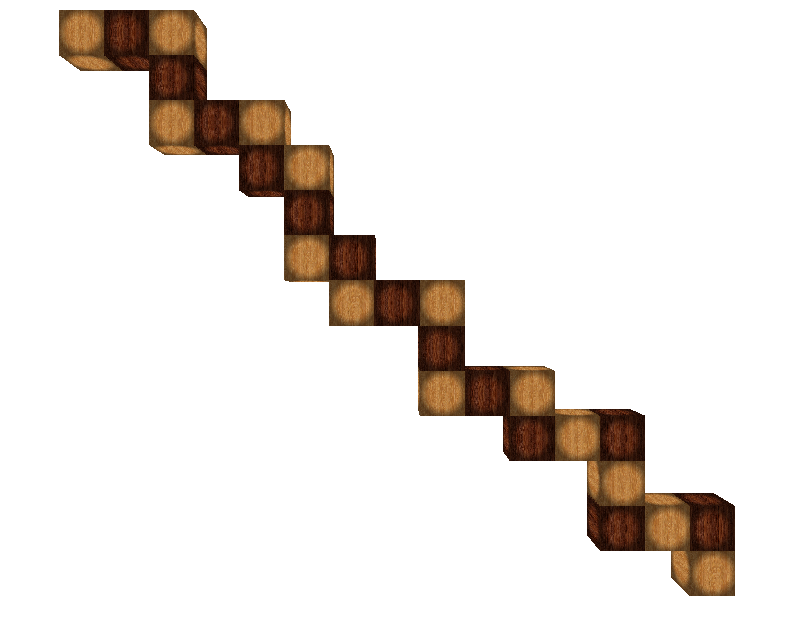
\includegraphics[width=0.7\textwidth]{start}
    \caption{Na zdjęciu widoczny ciąg połączonych ze sobą sześcianów – model w fazie początkowej.}
    \label{fig:joints1}
\end{figure}

\section{Przedstawienie łamigłówki w pamięci komputera}

Model zagadki konstruowany jest po dostarczeniu wektora długości poszczególnych fragmentów do aplikacji. Mniejsze sześciany umieszczane są w przestrzeni trójwymiarowej przez algorytm analizujący.

Między każdym łączeniem możliwy jest ruch rotacyjny, lecz nie każdy ruch jest znaczący dla stanu całego model. Wykonywanie ruchów w łączeniach nieznaczących jest redundantne, tj. uzyskanie stanu modelu po każdym możliwym obrocie w łączeniu nieznaczącym jest możliwe po wykonaniu ruchu na jednym z najbliższych łączeń znaczących. Przez analiza pokryte jest również wykrywanie połączeń znaczących.

\section{Cel zagadki}

Na podstawie wektora wejściowego obliczany jest najmniejszy bok sześcianu, w którym możliwe jest umieszczenie złożonego modelu. 

        \cleardoublepage

        \chapter{Projekt aplikacji}
\thispagestyle{chapterBeginStyle}
W rozdziale tym szczegółowo omówiono budowę aplikacji. Podano główny przebieg jej działania oraz opis komponentów, na które składa się program. Umieszczono również budowę algorytmów.

\section{Zastosowane technologie}
Aplikacja została napisana w języku C++ zgodnym ze standardem C++14\cite{Standard}. W celu zapewnienia czytelności kodu zastosowano niektóre zasady spisane w książce Roberta Martina \cite{CleanCode}.

\section{Główny tok działania}
Działanie aplikacji można podzielić na pięć głównych kroków. Każdy kolejny krok jest zależny od kroków poprzednich. Główny przebieg działania aplikacji złożony jest z następujących punktów:
\begin{enumerate}
\item Konstrukcja modelu na podstawie wektora wejściowego
\item Analiza modelu
\item Poszukiwanie wektora stanów modelu, który rozwiązującego łamigłówkę.
\item Poszukiwanie kombinacji ruchów rozwiązujących zadanie
\item Prezentacja wyników w postaci animacji 3D
\end{enumerate}

\section{Podział na moduły}
Aplikacja podzielona jest na zbiór komponentów, z których każdy odpowiedzialny jest za różne działania. Każdy z kroków głównego przebiegu jest rozparcelowany pomiędzy następujące segmenty:
\begin{enumerate}
\item Moduł opisu modelu.
\item Moduł kombinatoryczny.
\item Moduł geometryczny.
\item Moduł graficzny.
\end{enumerate}

\section{Moduł opisu modelu}
Zadaniem modułu jest przygotowanie danych dla głównego modułu rozwiązującego. Przetwarzane są w nim dane otrzymane bezpośrednio od użytkownika. Wynikiem jest reprezentacja modelu, która zostanie użyta w następnych krokach.

\textbf{Wejście:}
\begin{enumerate}
\item wektor długości fragmentów
\end{enumerate}

\textbf{Wyjście:}
\begin{enumerate}
\item wektor łączeń znaczących
\item wektor elementów w przestrzeni
\end{enumerate}

{\small
	\begin{pseudokod}[H]
	%\SetAlTitleFnt{small}
	\SetArgSty{normalfont}
	\KwIn{inputVector}
	\KwOut{elementPositions, jointsList}
    current $\leftarrow$ (x=0, y=0, z=0)\;
    side $\leftarrow$ 0\;
    Push current on elementPositions\;
    Push 0 on jointsList\;
    \ForEach{$p \in inputVector$}
    {
        \For{i $\leftarrow$ 1 \KwTo p-1}
        {
            \eIf{side == 1}
            {
                current.x $\leftarrow$ current.x + 1\;
            }
            {
                current.z $\leftarrow$ current.z + 1\;
            }
			Push current on elementPositions\;
        }
		Push (last element of jointsList + p - 1) on jointsList\;
        side $leftarrow$ 1 - side\;
    }
	\caption{Poszukiwanie wektora łączeń znaczących oraz wektora pozycji elementów w przestrzeni}
	\label{alg:mine3}
	\end{pseudokod}
}

Długość wektora łączeń znaczących jest równa długości wektora fragmentów. Wektor ten złożony jest ze wskaźników do elementów wektora elementów w przestrzeni, w których następuje 'załamanie' modelu.

\begin{figure}[h]
    \centering
    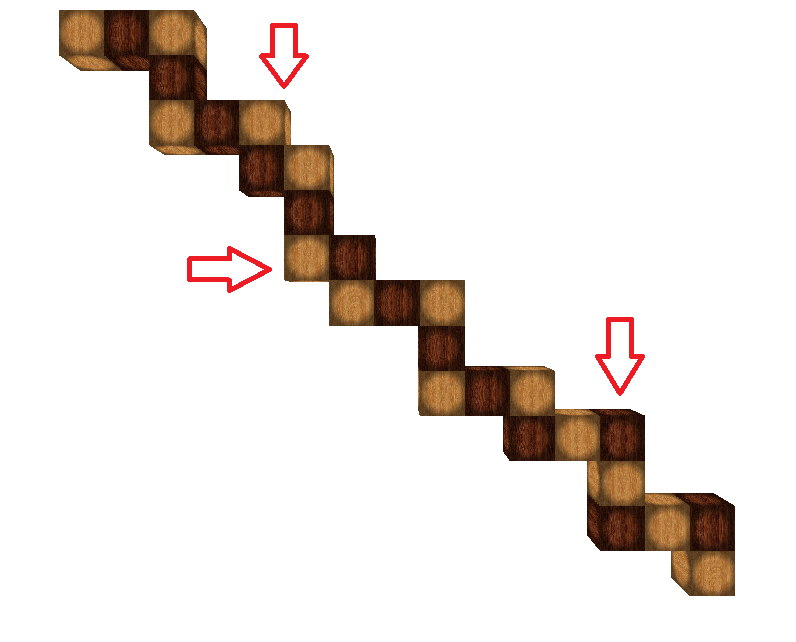
\includegraphics[width=0.7\textwidth]{joints}
    \caption{Przykładowe łączenia mające znaczenie w czasie rozwiązywania łamigłówki, wskazane przez czerwone strzałki.}
    \label{fig:joints1}
\end{figure}

Wektor elementów w przestrzeni złożony jest z punktów (złożonych ze współrzędnych x, y oraz z) wskazujących na środki mniejszych sześcianów rozmieszczonych w przestrzeni. W każdym stanie, w jakim znajdzie się cały model, wektor ten skonstruowany jest tak, by kolejne elementy były oddalone od siebie o wartość 1 względem jednej z osi OX, OY albo OZ.

\begin{center}
$\sqrt{(x_i - x_{i+1})^2 + (y_i - y_{i+1})^2 + (z_i - z_{i+1})^2} = 1$,

$|x_i - x_{i+1}| = 1  \oplus  |y_i - y_{i+1}| = 1  \oplus  |z_i - z_{i+1}| = true$,

$i \in \{ 1, 2, \ldots, length(elements)-1 \}$
\end{center}

\section{Moduł kombinatoryczny}
Zadaniem modułu jest znalezienie rozwiązania łamigłówki, tj. kombinacji takich ruchów, które w sposób prawidłowy doprowadzą do ułożenia zagadki. Działanie modułu składa się z dwóch następujących po sobie faz:

\begin{enumerate}
\item Faza pierwsza: Poszukiwanie wektora rozwiązującego łamigłówkę.
\item Faza druga: Poszukiwanie kombinacji ruchów dążących do otrzymania wektora rozwiązującego łamigłówkę.
\end{enumerate}

\subsection{Faza pierwsza}
\textbf{Wejście:}
\begin{enumerate}
\item wektor łączeń znaczących
\item wektor elementów w przestrzeni
\end{enumerate}

\textbf{Wyjście:}
\begin{enumerate}
\item wektor rozwiązujący łamigłówkę
\end{enumerate}

{\small
	\begin{pseudokod}[H]
	%\SetAlTitleFnt{small}
	\SetArgSty{normalfont}
	\SetKwFunction{rotatePartOfModel}{rotatePartOfModel}
	\SetKwFunction{checkThatCollisionsNotOccureAfterRotation}{checkThatCollisionsNotOccureAfterRotation}
	\SetKwProg{Fn}{Function}{}{}
	\SetKwFunction{checkThatCurrentModelPartFitRequirement}{checkThatCurrentModelPartFitRequirement}
	\SetKwFunction{searchForResultState}{searchForResultState}
	\Fn{searchForResultState($elements, joint, inCube$)}
	{
		\For{$i \leftarrow 0$ \KwTo $3$}
		{
			combinationVector[joint] $\leftarrow$ (combinationVector[joint] + 1) mod 4\;
			\rotatePartOfModel{joint, pi/2}\;
			\If{\checkThatCollisionsNotOccureAfterRotation{$elements,joint$} = true}
			{
				\If{\checkThatCurrentModelPartFitRequirement{$elements, joint, inCube, outCube$} = true}
				{
					\eIf{$joint$ = $modelSize$ - 2}
					{
						\Return true
					}
					{
						\If{\searchForResultState{$elements, joint + 1, outCube$} = true}
						{
							\Return true
						}
					}
				}
			}
		}
		combinationVector[joint] $\leftarrow$ 0\;
		\Return false
	}
	\caption{Poszukiwanie wektora rozwiązującego łamigłówkę}\label{alg:mine}
	\end{pseudokod}
}

W powyższym pseudokodzie użyte zostały następujące procedury:
\begin{itemize}
\item rotatePartOfModel - obraca część łamigłówki od jej początku do podanego łączenia.
\item checkThatCollisionsNotOccureAfterRotation - sprawdza czy żadne dwa elementy od początku do podanego łączenia po obróceniu nie znajdują się w tej samej pozycji.
\item checkThatCurrentModelPartFitRequirement - sprawdza czy część modelu od jego początku do podanego łączenia spełnia ograniczenia modelu.
\end{itemize}

\clearpage 

\subsection{Faza druga}

W fazie drugiej znajdowana jest permutacja ruchów rozwiązująca zagadkę. W algorytmie tym ważną kwestią jest unikanie kolizji w czasie wykonywania kolejnych ruchów. Istotne jest zatem wykrywanie i zapobieganie kolizjom w każdym stanie modelu oraz w fazach przejścia między kolejnymi stanami. Algorytm wykrywający kolizje w czasie danego ruchu opiera swoje działanie o szereg działań algebraicznych, których skutkiem jest odpowiedź na pytanie, czy w czasie wykonania danego ruchu nastąpi kolizja.

\textbf{Wejście:}
\begin{enumerate}
\item wektor rozwiązujący łamigłówkę
\item zbiór łączeń znaczących
\item zbiór elementów rozmieszczonych w przestrzeni
\end{enumerate}
\textbf{Wyjście:}
\begin{enumerate}
\item wektor kombinacji ruchów
\end{enumerate}
{\small
	\begin{pseudokod}[H]
	%\SetAlTitleFnt{small}
	\SetArgSty{normalfont}
	\SetKwFunction{tryToRotate}{tryToRotate}
	\KwIn{permutation}
	\KwOut{endPermutation}
	loopBreak = false\;
    \While{loopBreak = false}
    {
        \For{x $\leftarrow$ 0 \KwTo length(permutation)-1}
        {
            \If{NOT(\tryToRotate{permutation[x].joint, permutation[x].move} = true}
            {
                \For{y $\leftarrow$ x+1 \KwTo length(permutation)}
                {
                    temp $\leftarrow$ permutation[x]\;
                    permutation[x] $\leftarrow$ permutation[y]\;
                    permutation[y] $\leftarrow$ temp\;
                    \If{\tryToRotate{permutation[x].joint, permutation[x].move} = true}
                    {
						Continue Outter For Loop\;
					}
                }
                rr $\leftarrow$ (random integer) mod x\;
                temp $\leftarrow$ permutation[x]\;
                permutation[x] $\leftarrow$ permutation[rr]\;
                permutation[rr] $\leftarrow$ temp\;
                Continue While Loop\;
            }
        }
		loopBreak $\leftarrow$ true\;
    }
	endPermutation $\leftarrow$ permutation\;
	\caption{Poszukiwanie wektora permutacji ruchów rozwiązującej łamigłówkę}\label{alg:mine}
	\end{pseudokod}
}

W powyższym pseudokodzie użyto procedury tryToRotate. Procedura zwraca wartość 'true' jeśli udało się obrócić część modelu od jej początku do podanego łączenia, bądź false w przeciwnym razie. Procedura w przypadku powodzenia zmienia stan wektora elementów rozmieszczonych w przestrzeni.

W procedurze tej poszukiwana jest odpowiednia kombinacja ruchów. Pętla while kończy swoje działanie po znalezieniu kombinacji. Pierwsza pętla for sprawdza czy dana kombinacja spełnia warunki modelu. Jeśli w którymś momencie nastąpi ruch wywołujący kolizję, następuje procedura poszukiwania ruchu jeszcze niewykonanego, który po zamianie z bieżącym ruchem pozwoli kontynuować działanie pętli. Jeśli taki ruch nie zostanie znaleziony to oznacza, że kombinacja ruchów $0,1,\ldots,x$ mimo spełnienia założeń o braku kolizji nie pozwoli na rozwiązanie łamigłówki. W takiej sytuacji algorytm niedeterministycznie zamienia miejscami aktualnie badany ruch (wywołujący kolizję) z jednym z poprzednich ruchów. Dzieje się tak dlatego, że aktualnie badany ruch $permutation[x]$ musi zostać wykonany przed jednym z już zbadanych ruchów.

\section{Moduł geometryczny}
Moduł geometryczny jest zbiorem funkcjonalności pomocniczych, wykorzystywanych w pozostałych komponentach. Odpowiedzialny jest za skomplikowane obliczenia matematyczne, takie jak przewidywanie kolizji w czasie ruchu, stwierdzanie kolizji po wykonanym ruchu itp. Jednym z ważniejszych algorytmów jest wyszukiwanie zaistniałych kolizji.

{\small
	\begin{pseudokod}[H]
	%\SetAlTitleFnt{small}
	\SetArgSty{normalfont}
	\KwIn{model, joint, cubeIn}
	\KwOut{cubeOut}
	\eIf{joint + 2 $<$ length(jointsList)}
	{
		elementsToCheck $\leftarrow$ jointsList[joint + 2]
	}
	{
		elementsToCheck $\leftarrow$ last element of jointSet
	}
		
	\For{$i \leftarrow jointsList[joint] $ \KwTo elementsToCheck}
	{
		\If{model[i].x $<$ cubeIn.minX}
		{
			cubeOut.minX $\leftarrow$ model[i].x
		}
		\If{model[i].y $<$ cubeIn.minY}
		{
			cubeOut.minY $\leftarrow$ model[i].y
		}
		\If{model[i].z $<$ cubeIn.minZ}
		{
			cubeOut.minZ $\leftarrow$ model[i].z
		}
		\If{model[i].x $>$ cubeIn.maxX}
		{
			cubeOut.maxX $\leftarrow$ model[i].x
		}
		\If{model[i].y $>$ cubeIn.maxY}
		{
			cubeOut.maxY $\leftarrow$ model[i].y
		}
		\If{model[i].z $>$ cubeIn.maxZ}
		{
			cubeOut.maxZ $\leftarrow$ model[i].z
		}
	}
	\eIf{outCube.maxX - outCube.minX $<$ cubeSize OR outCube.maxY - outCube.minY $<$ cubeSize OR outCube.maxZ - outCube.minZ $<$ cubeSize}
	{
		\Return false
	}
	{
		\Return true
	}
	\caption{Badanie wystąpienia kolizji po wykonanej rotacji od początku modelu do łączenia $joint$}\label{alg:mine}
	\end{pseudokod}
}

Algorytm wykorzystywany jest w fazie pierwszej, patrz Pseudokod 3.2.

\section{Moduł graficzny}
Komponent odpowiedzialny jest za obsługę wyświetlania grafiki, zarządzaniem animacją oraz obsługę zdarzeń klawiatury i myszy. Biblioteką graficzną wykorzystywaną przez ten komponent jest zestaw OpenGL\cite{OpenGL}.
Wejściem dla komponentu są:
\begin{enumerate}
\item zbiór łączeń znaczących
\item zbiór elementów rozmieszczonych w przestrzeni
\item wektor kombinacji ruchów rozwiązujących zadanie
\end{enumerate}

Wyjściem komponentu jest interaktywna trójwymiarowa animacja wyświetlana w środowisku użytkownika. 

Sposób przedstawienia rozwiązania jest możliwie jak najbardziej przystępny dla przeciętnego człowieka. Dzięki interaktywnej animacji komputerowej analiza każdego ruchu jest ułatwiona dla użytkownika. W rozdziale 4. omówione jest sterowanie programem oraz przykładowe zdjęcie przedstawiające działanie modułu graficznego.

        \cleardoublepage

        \chapter{Działanie programu}
\thispagestyle{chapterBeginStyle}

\section{Instalacja}

Do poprawnego działania aplikacji wymagany jest system operacyjny wspierający zestaw bibliotek OpenGL. Rozważa się dwie możliwości instalacji:
\begin{enumerate}
\item Użycie pre-kompilowanego pliku wykonywalnego, skompilowanego na odpowiednią platformę.
\item Własnoręczna kompilacja przy użyciu polecenia 'make', przy czym należy spełnić następujące wymagania: 
	\begin{itemize}
	\item Kompilator g++ wspierający standard C++14
	\item Zainstalowane w systemie programistyczne biblioteki z zestawu OpenGL
	\item Zainstalowane w systemie programistyczne biblioteki z zestawu freeglut
	\item Narzędzie obsługujące pliki typu Makefile (np. linuxowy 'make')
	\end{itemize}
\end{enumerate}

\section{Dane wejściowe}

Wymagany jest przez aplikację zewnętrzny plik z opisem modelu w formacie {liczba1,liczba2,liczba3,\ldots}. Kolejne liczby oznaczają kolejne długości fragmentów, z których złożony jest model. Ścieżkę do wspomnianego pliku należy podać do standardowego wejścia programu. Po uruchomieniu plik wczytywany jest przez aplikację i następuje generowanie modelu.

\section{Poszukiwanie rozwiązywania}

Po poprawnym wygenerowaniu modelu następuje proces jego rozwiązywania. Ze względu na złożoność algorytmów może on potrwać od ułamka sekund aż do czasu bliżej nieokreślonego. Czas rośnie wraz ze złożonością modelu, tj. liczbą łączeń znaczących.

\section{Prezentacja wyniku}

Wynik przedstawiony jest w postaci interaktywnej animacji komputerowej.

Sterowanie klawiaturą:
\begin{itemize}
\item 'W' - przybliżenie modelu
\item 'S' - oddalenie modelu
\item 'N' - następny ruch
\item 'P' - poprzedni ruch
\end{itemize}

Obsługiwane są również zdarzenia pochodzące od myszy (touchpada, \ldots). Poruszanie myszą z przyciśniętym lewym klawiszem myszy daje możliwość obracania modelu pod dowolnym kątem. Dzięki temu użytkownik jest w stanie dokładnie przyjrzeć się modelowi zarówno w stanie spoczynku, jak i podczas wykonywania przez program obrotów.

\begin{figure}[h]
    \centering
    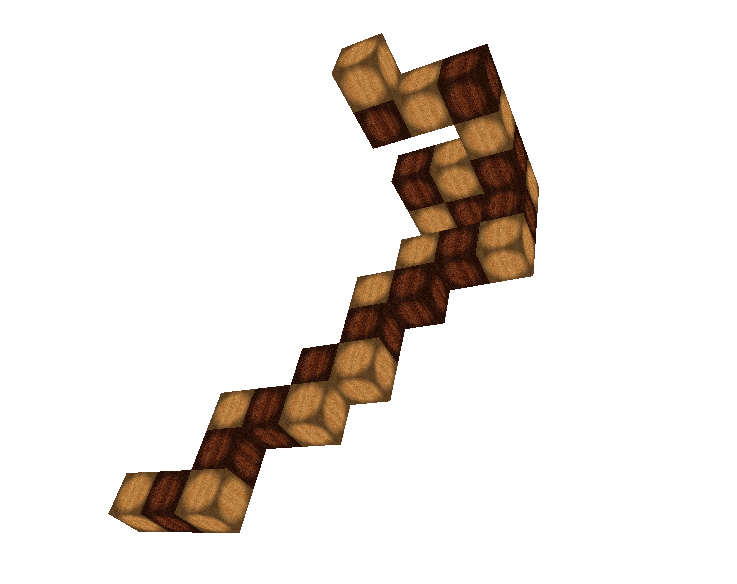
\includegraphics[width=0.7\textwidth]{using}
    \caption{Przykładowy zrzut ekranu wykonany w czasie działania programu}
    \label{fig:using1}
\end{figure}
        \cleardoublepage

        \chapter{Analiza algorytmów}
\thispagestyle{chapterBeginStyle}

Rozdział ten jest skupiony wokół analizy głównych algorytmów rozwiązujących łamigłówkę. Algorytmy pomocnicze nie są brane pod uwagę ze względu na swoją prostotę oraz mniejsze znaczenia dla działania systemu. Ośrodkiem najważniejszych algorytmów aplikacji jest moduł kombinatoryczny. Algorytmy przeanalizowano pod kątem pesymistycznego czasu działania\cite{Algorithms}. Przeprowadzono eksperymenty obliczeniowe, uzyskane średnie czasy obliczeń umieszczono w tabeli na końcu rozdziału.

Jak zostało wspomniane w rozdziale 2. działanie modułu kombinatorycznego oparte jest na dwóch niezależnych fazach.

W fazie pierwszej (Pseudokod 3.2) przeszukiwane jest drzewo dopuszczalnych kombinacji, w jakich może znaleźć się model. W czasie każdego kroku sprawdzane jest, czy aktualny stan jest poprawny, tj. czy do aktualnego ruchu badana część modelu znajduje się w stanie akceptującym. Stan akceptujący objawia się prawidłowym rozmieszczeniem elementów:
\begin{itemize}
\item brak kolizji,
\item elementy nie są poza granicami dopuszczalnymi przez cel łamigłówki (sześcian o odpowiednim boku).
\end{itemize}

Pesymistyczna złożoność obliczeniowa jest rzędu: $ O(4^{n}) $,

Złożoność pamięciowa: $ O(n) $ , gdzie n oznacza ilość łączeń znaczących.

Jednakże, dzięki zastosowanym ograniczeniom ilość możliwych kombinacji diametralnie maleje. Wiąże się to ze wczesnym wykrywaniem krawędzi przeszukiwanego drzewa, które z pewnością nie doprowadzą do poprawnego wyniku. Możliwe jest to dzięki sprawdzaniu spełnienia wymagań postawionych przed modelem oraz wykrywania zaistniałych kolizji w każdym kroku przeszukiwania. Pozwala to na rozwiązanie łamigłówki składającej się z około 70 łączeń znaczących (kostka o boku długości sześciu mniejszych sześcianów) w czasie sięgającym kilkunastu minut na przeciętnym komputerze. 

Faza druga (Pseudokod 3.3) jest odpowiedzialna za obliczenie wektora ruchów doprowadzających do rozwiązania łamigłówki. Poszukiwana jest permutacja ruchów. Obliczanie wspomnianego wektora jest związane z losowym rozmieszczaniem kolejności ruchów, do czasu gdy dana kombinacja rozwiąże łamigłówkę. Zastosowano również zabieg przyspieszający poszukiwania. Pesymistyczny czas takiego postępowania wydaje się być nieakceptowalny, jednakże doświadczalnie pokazane jest, że ciąg ruchów stosunkowo szybko osiąga pożądaną kolejność.

Pesymistyczna złożoność obliczeniowa jest rzędu: $ O(n!/k) $,

Złożoność pamięciowa: $ O(n) $, gdzie n oznacza ilość łączeń znaczących, k oznacza ilość permutacji rozwiązujących zadanie.

Pesymistyczny czas wskazuje na bardzo niską optymalizację fazy drugiej. Jednakowoż liczba kombinacji rozwiązujących zagadkę rośnie wraz ze wzrostem jej złożoności, stąd prawdopodobieństwo uzyskania prawidłowej permutacji w stosunkowo krótkim czasie jest wysoka.



W poniższej tabelce przedstawiono średnie czasy rozwiązywania łamigłówek różnych rozmiarów:
\begin{center}
\begin{tabular}{|c|r|r|}
\hline
{\bf Rozmiar} & {\bf Liczba łączeń znaczących} & {\bf Czas rozwiązania (sek.)} \\
\hline
\hline
$2\times 2\times 2$ & $7$ & $0.0002$ \\
\hline
$3\times 3\times 3$ & $16$ & $0.0016$ \\
\hline
$4\times 4\times 4$ & $38$ & $1.8476$ \\
\hline
$5\times 5\times 5$ & $49$ & $3.1958$ \\
\hline
$6\times 6\times 6$ & $71$ & $309.4230$ \\
\hline
$7\times 7\times 7$ & $97$ & Przerwano po 30 minutach \\
\hline
\end{tabular}
\end{center}
        \cleardoublepage

        \chapter{Podsumowanie}
\thispagestyle{chapterBeginStyle}

W aplikacji rozwiązującej łamigłówki geometryczne użyto połączenia dwóch nowatorskich algorytmów, które wykorzystując wykrywanie kolizji, są w stanie znajdować kombinację ruchów w celu rozwiązania zadania. Użytkownik naśladując zachowanie programu jest zdolny do rozwiązania tego typu problemów, nie znając technik ich rozwiązywania. Wyświetlanie grafiki trójwymiarowej wspieranej biblioteką OpenGL daje w rezultacie przyjazną dla użytkownika aplikację. Wieloplatformowość wspomnianej biblioteki pozwala na uruchomienie programu w każdym środowisku, które jest przez nią wspierane. Prawdopodobnie niewiele jest aplikacji pozwalających rozwiązywać tego typu łamigłówki. Z dużym prawdopodobieństwiem graniczącycm z pewnośią nie są one w tej chwili na tyle popularne, by dotarły do każdego potencjalnego użytkownika.

Jednakże algorytmy te wymagają ulepszenia. Pesymistyczny czas fazy pierwszej przekreśla szansę na rozwiązanie większości łamigłówek o wynikowym sześcianie długości powyżej 6 mniejszych kostek. Być może praktyczne wprowadzenie paradygmatu ,,constraints programming'' (w wolnym tłumaczeniu: programowania ograniczeniami) pozwoliłoby na uzyskanie znacząco lepszych rezultatów. Dodatkowo algorytm fazy drugiej należy poddać wnikliwej analizie średniej złożoności obliczeniowej oraz niezawodności w znajdowaniu rozwiązania.

        \cleardoublepage


        %%%%%%%%%%%%%%%%%%%%%%%%%%%%%%%%%%%%%%%%%%%%%%%%%%%%%%%%%%%%%%%%%%%%%%%%%%%%%%
        %%%%%%%%%%%%%%%%%%%%%%%%%%%%%%% BIBLIOGRAFIA %%%%%%%%%%%%%%%%%%%%%%%%%%%%%%%%%
        %%%%%%%%%%%%%%%%%%%%%%%%%%%%%%%%%%%%%%%%%%%%%%%%%%%%%%%%%%%%%%%%%%%%%%%%%%%%%%

        \pagestyle{bibliographyStyle}
        \bibliographystyle{plabbrv}
        \bibliography{literatura}
        \thispagestyle{chapterBeginStyle}
        \addcontentsline{toc}{chapter}{Bibliografia}

        \cleardoublepage

        %%%%%%%%%%%%%%%%%%%%%%%%%%%%%%%%%%%%%%%%%%%%%%%%%%%%%%%%%%%%%%%%%%%%%%%%%%%%%%
        %%%%%%%%%%%%%%%%%%%%%%%%%%%%%%%%% DODATKI %%%%%%%%%%%%%%%%%%%%%%%%%%%%%%%%%%%%
        %%%%%%%%%%%%%%%%%%%%%%%%%%%%%%%%%%%%%%%%%%%%%%%%%%%%%%%%%%%%%%%%%%%%%%%%%%%%%%

        \appendix
        \pagestyle{appendixStyle}

        \chapter{Zawartość płyty CD}
\thispagestyle{chapterBeginStyle}
\label{plytaCD}

Płyta CD zawiera:
\begin{itemize}
\item Pracę dyplomową w formie elektronicznej.
\item Kody źródłowe aplikacji, plik Makefile oraz pliki graficzne, potrzebne do prawidłowego funkcjonowania aplikacji.
\end{itemize}

        \cleardoublepage

\end{document}

